
\subsection{Particle Beam Requirements}
The requested beam parameters are driven by the requirement that the results from the CERN test beam should be directly applicable to the future large underground single-phase LAr detector with minimal extrapolation. The CERN test beam data will be used to evaluate the detector performance, to understand the various physics systematic effects, and to provide ``neutrino-like'' data for event reconstruction studies. To satisfy the requirement, the beam parameters must span a broad range of particle spectrum that are expected in the future neutrino experiment. The particle beam composition should consist of electrons, muons, and hadron beams that are charge-selected. The expected momentum distributions for secondary particles from neutrino interactions are shown earlier in Figure~\ref{fig:particle_momenta}. There is a large spread in the momentum distribution with most particles peaked near 200 MeV/c. To cover the momentum range of interest, the momentum of the test beam should step from 0.2 GeV/c to 7 GeV/c. The maximum electron drift time in the TPC is about 2.2 ms. To minimize pile-up in the TPC, the desired beam rate should be around 200 Hz. The single-phase TPC consists of two drift volumes. It is desirable to aim the particle beam so that the hadronic showers are mostly contained in the same drift volume.  However, we also plan to take some data with the beam entering different region of the TPC, and may include some data with particles crossing one drift volume to the next. %The two beam entry angles and positions with respect to the LAr cryostat are shown in Figures \ref{fig:BP_SideView} and \ref{fig:BP_TopView}. 
The beam nominally enters the cryostat slightly downward at an angle of about 6 degrees. Along the horizontal plane, the beam enters the cryostat with an angle of 10 degrees. The summary of the beam requirements are shown in Table~\ref{table:beamspecs}.

%\begin{figure}[h]
%  \centering
%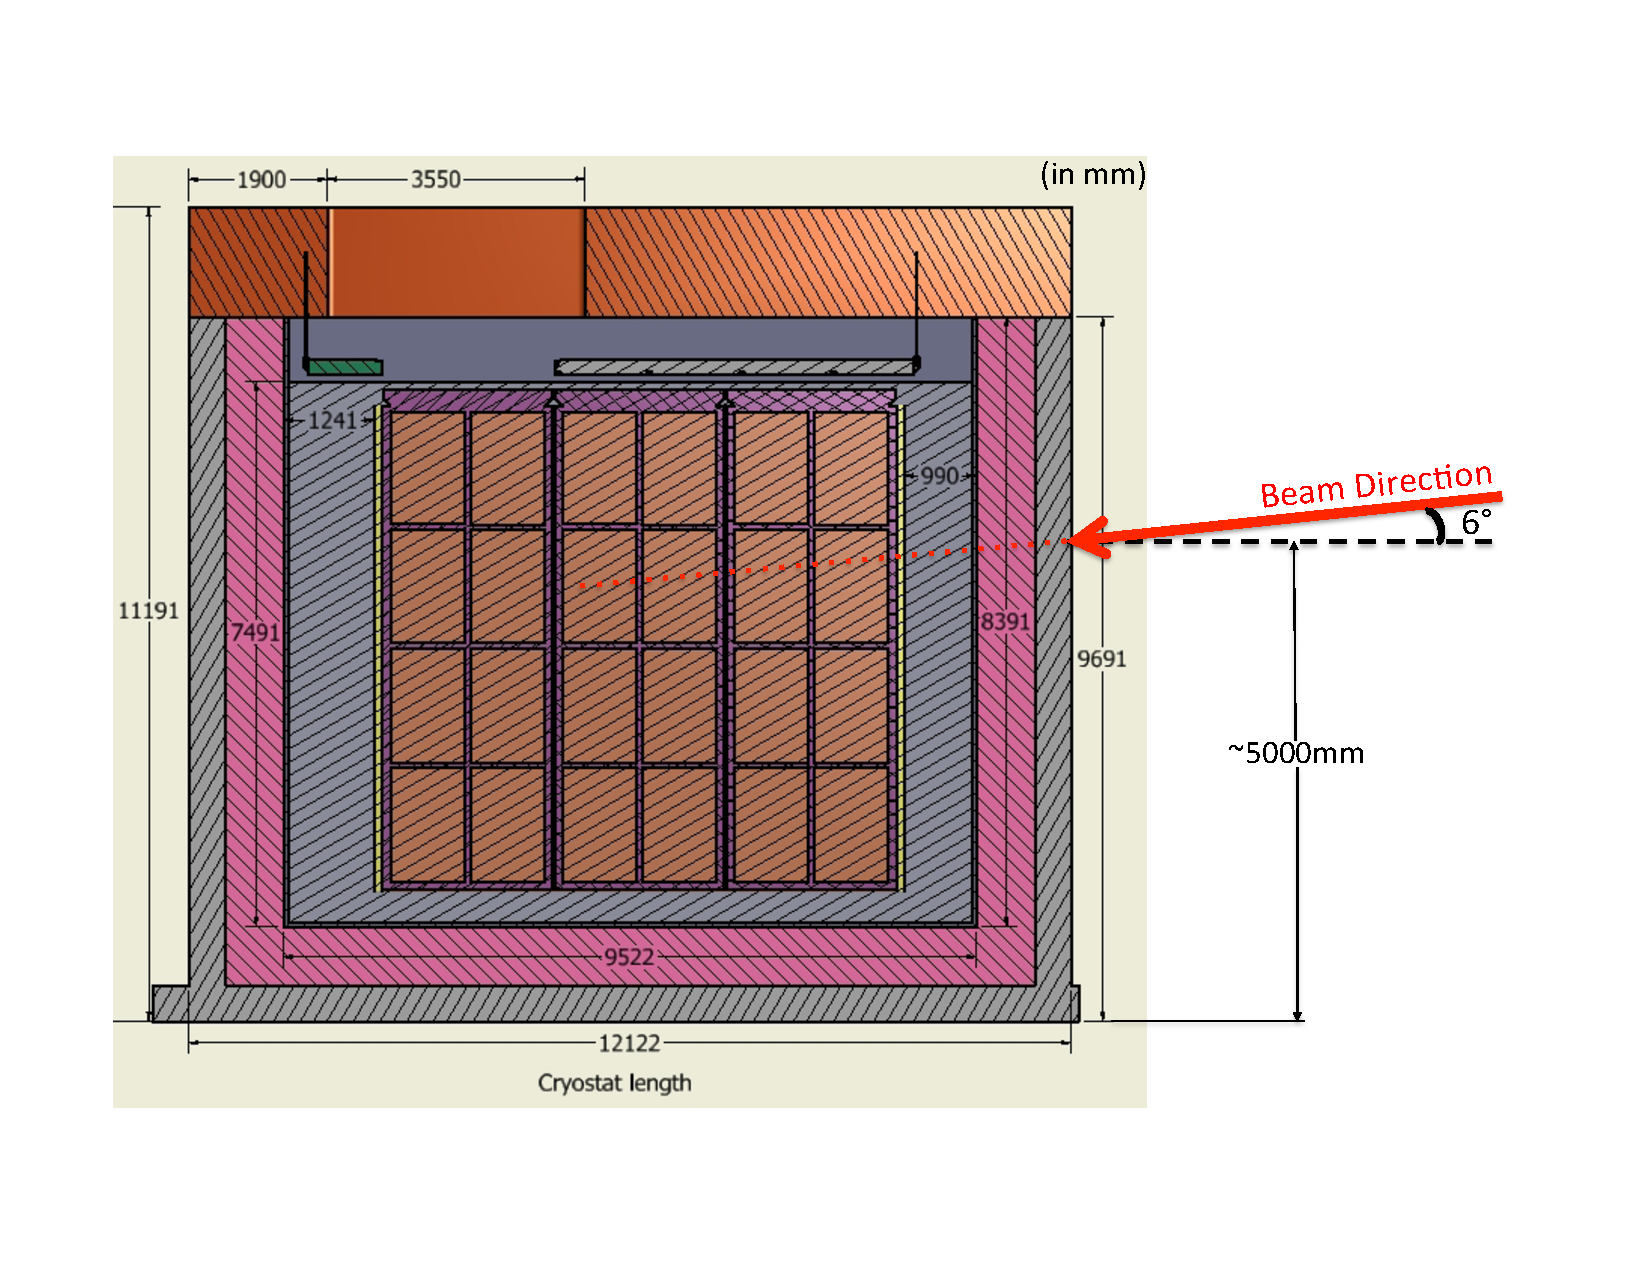
\includegraphics[scale=0.6]{figures/BeamPos_SideView.pdf}
%  \caption{Side view: beam enters the cryostat slightly downward with a dip angle of 6 degrees.  }
%  \label{fig:BP_SideView}
%\end{figure}
%
%\begin{figure}[h]
%  \centering
%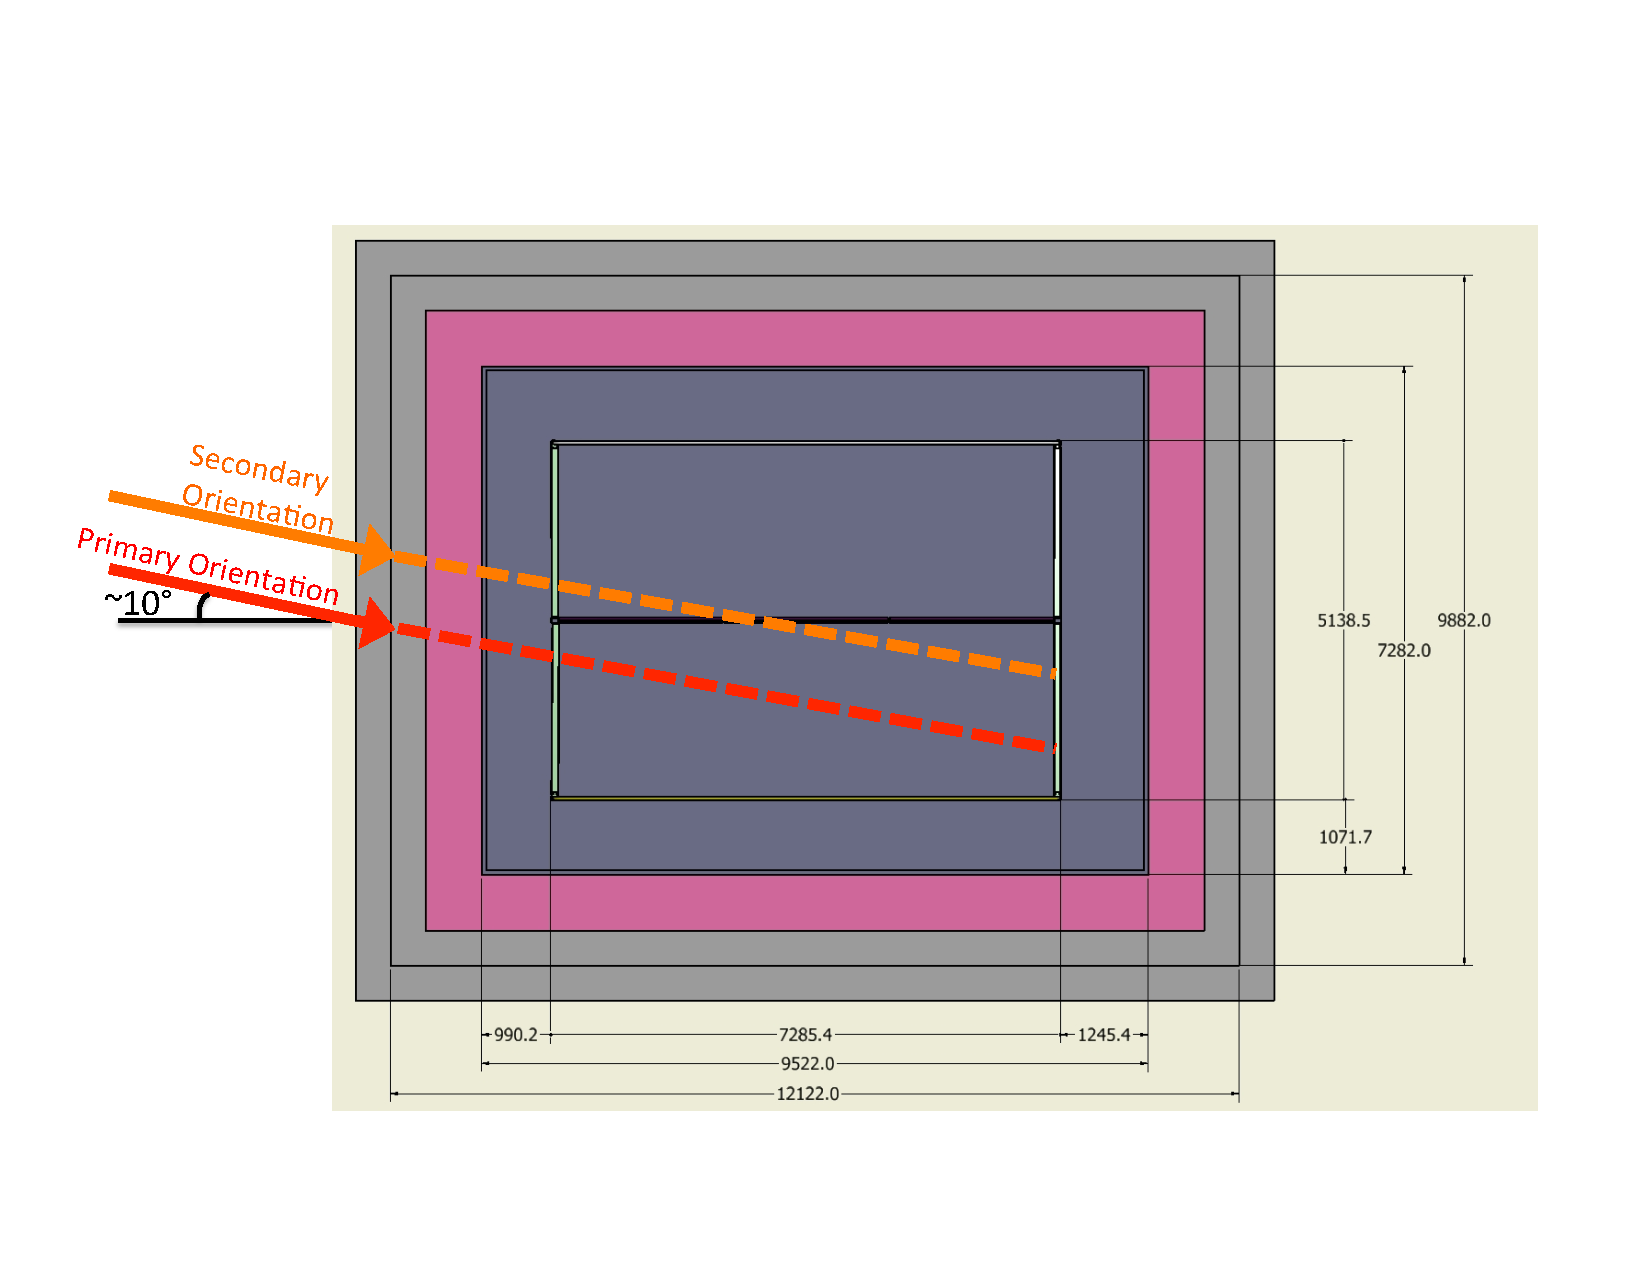
\includegraphics[scale=0.6]{figures/BeamPos_TopView.pdf}
%  \caption{Top view: beam enters the cryostat with an entry angle of about 10 degrees along the horizontal plane. The primary orientation sends the particle beam into one TPC drift volume. The secondary oritentation sends the particle beam across the APA. }
%  \label{fig:BP_TopView}
%\end{figure}

\begin{table}[h]
\centering
\begin{tabular}{|c|c|}
\hline
\textbf{Parameter } & \textbf{Requirements}  \\ \hline
  Particle Types        & $e^\pm,\mu^\pm,\pi^\pm$  \\ \hline
  Momentum Range   & 0.2 - 7 GeV/$c$ \\ \hline
  Momentum Spread   & $\Delta p/p  < $5 \%   \\ \hline
  Transverse Beam Size   & RMS(x,y) $\approx$ 10 cm  \\
  & (At the entrance face of the LAr cryostat) \\ \hline
  Beam Divergence & tbd   \\ \hline
  Beam Angle &  $\approx10^{\circ}$    \\
  (horizontal plane) &  \\ \hline
  Beam Dip Angle &  -6$^\circ$ (nominal); $\pm5^\circ$ range    \\ 
  (vertical plane) &  \\ \hline
  Beam Entrance Position & Multiple beam windows    \\ \hline
  Rates & 200 Hz (maximum)    \\ \hline
\end{tabular}
\caption{Particle beam requirements.}
\label{table:beamspecs}
\end{table}

\subsection{EHN1 H4ext Beamline}
The H4ext is an extension of the existing H4 beamline in Experimental Hall North 1 (EHN1).  To produce particles in the momentum range of interest, 60 - 80 GeV/c pion beam from the T2 target is used to generate tertiary beams. The tertiary particles are momentum and charge-selected and transported down H4ext beamline to the experimental area. A conceptual layout of the H4ext beamline is shown in Figure~\ref{fig:H4extPrelim}.  In the Figure, the cryostat for this proposal is located at the lower right hand corner of the plot. The cryostat in the upper left is for the WA105 Collaboration.

\begin{figure}[h]
  \centering
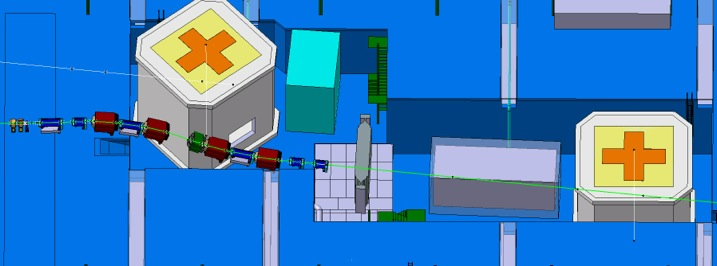
\includegraphics[scale=0.7]{figures/EHN1Ext_Prelim.jpg}
  \caption{A conceptual layout of the H4ext beamline  }
  \label{fig:H4extPrelim}
\end{figure}

%\subsubsection{Beam Optics}
%[Waiting for inputs from Ilias]

\subsection{Beam Instrumentation}
Beam instrumentation provides important information about the characteristics of the beam. It is expected that a series of detectors will be installed along the beam line to measure the particle momentum, identify particle type, and track the particle trajectory.

\subsubsection{Beam Position Detector}
The beam position detector measures the positions of the particle as it traverses the detector. Two detector technologies are under considerations: wire chambers and scintillating fiber trackers. For the nominal setup, one beam position detector is installed upstream and another one downstream of the last bending magnet. This pair provides additional momentum information about the particiles as well as the first set of position measurements. A third detector is placed right in front of the beam window on the cryostat wall to provide the last position information before the beam enters the cryostat.

\subsubsection{Particle Identification}
In order to have good particle identification over large momentum range, two indepent particle identfication systems are needed in the beamline. The Time-of-Flight system will be used to cover lower momentum range while a Threshold Cherenkov detector will be tuned for higher momentum particles.

\subsubsection{Muon Beam Halo Counters}
The halo counter is a set of plastic scintillator paddles surrounding the beamline. The main purpose is to tag particles (primarily muons from the upstream production target) that are outside of the beam axis, but may potentially enter the TPC volume. The counter information is used to either veto or simply flag these class of events.

%\subsection{Beam Window on LAr Cryostat}
%This section could be absorbed into the cryostat chapter.


\subsection{Beam Rates and Run Plan}
At the time of this proposal, the beamline design has not been finalized. To estimate the beam rates, we use inputs from a generic target simulation based on 100K 80 GeV $\pi^+$ beam on 15 cm copper target. This $\pi^+$ rate is roughly equivalent to 10\% of a typical SPS spill. The distributions of the tertiary particles from the copper target are shown in Figure~\ref{fig:PionOnCuTarget}. The figure on the left is for postively charged and the figure on the right is for negatively charged tertiary particles. 

\begin{figure}[tbh]
  \centering
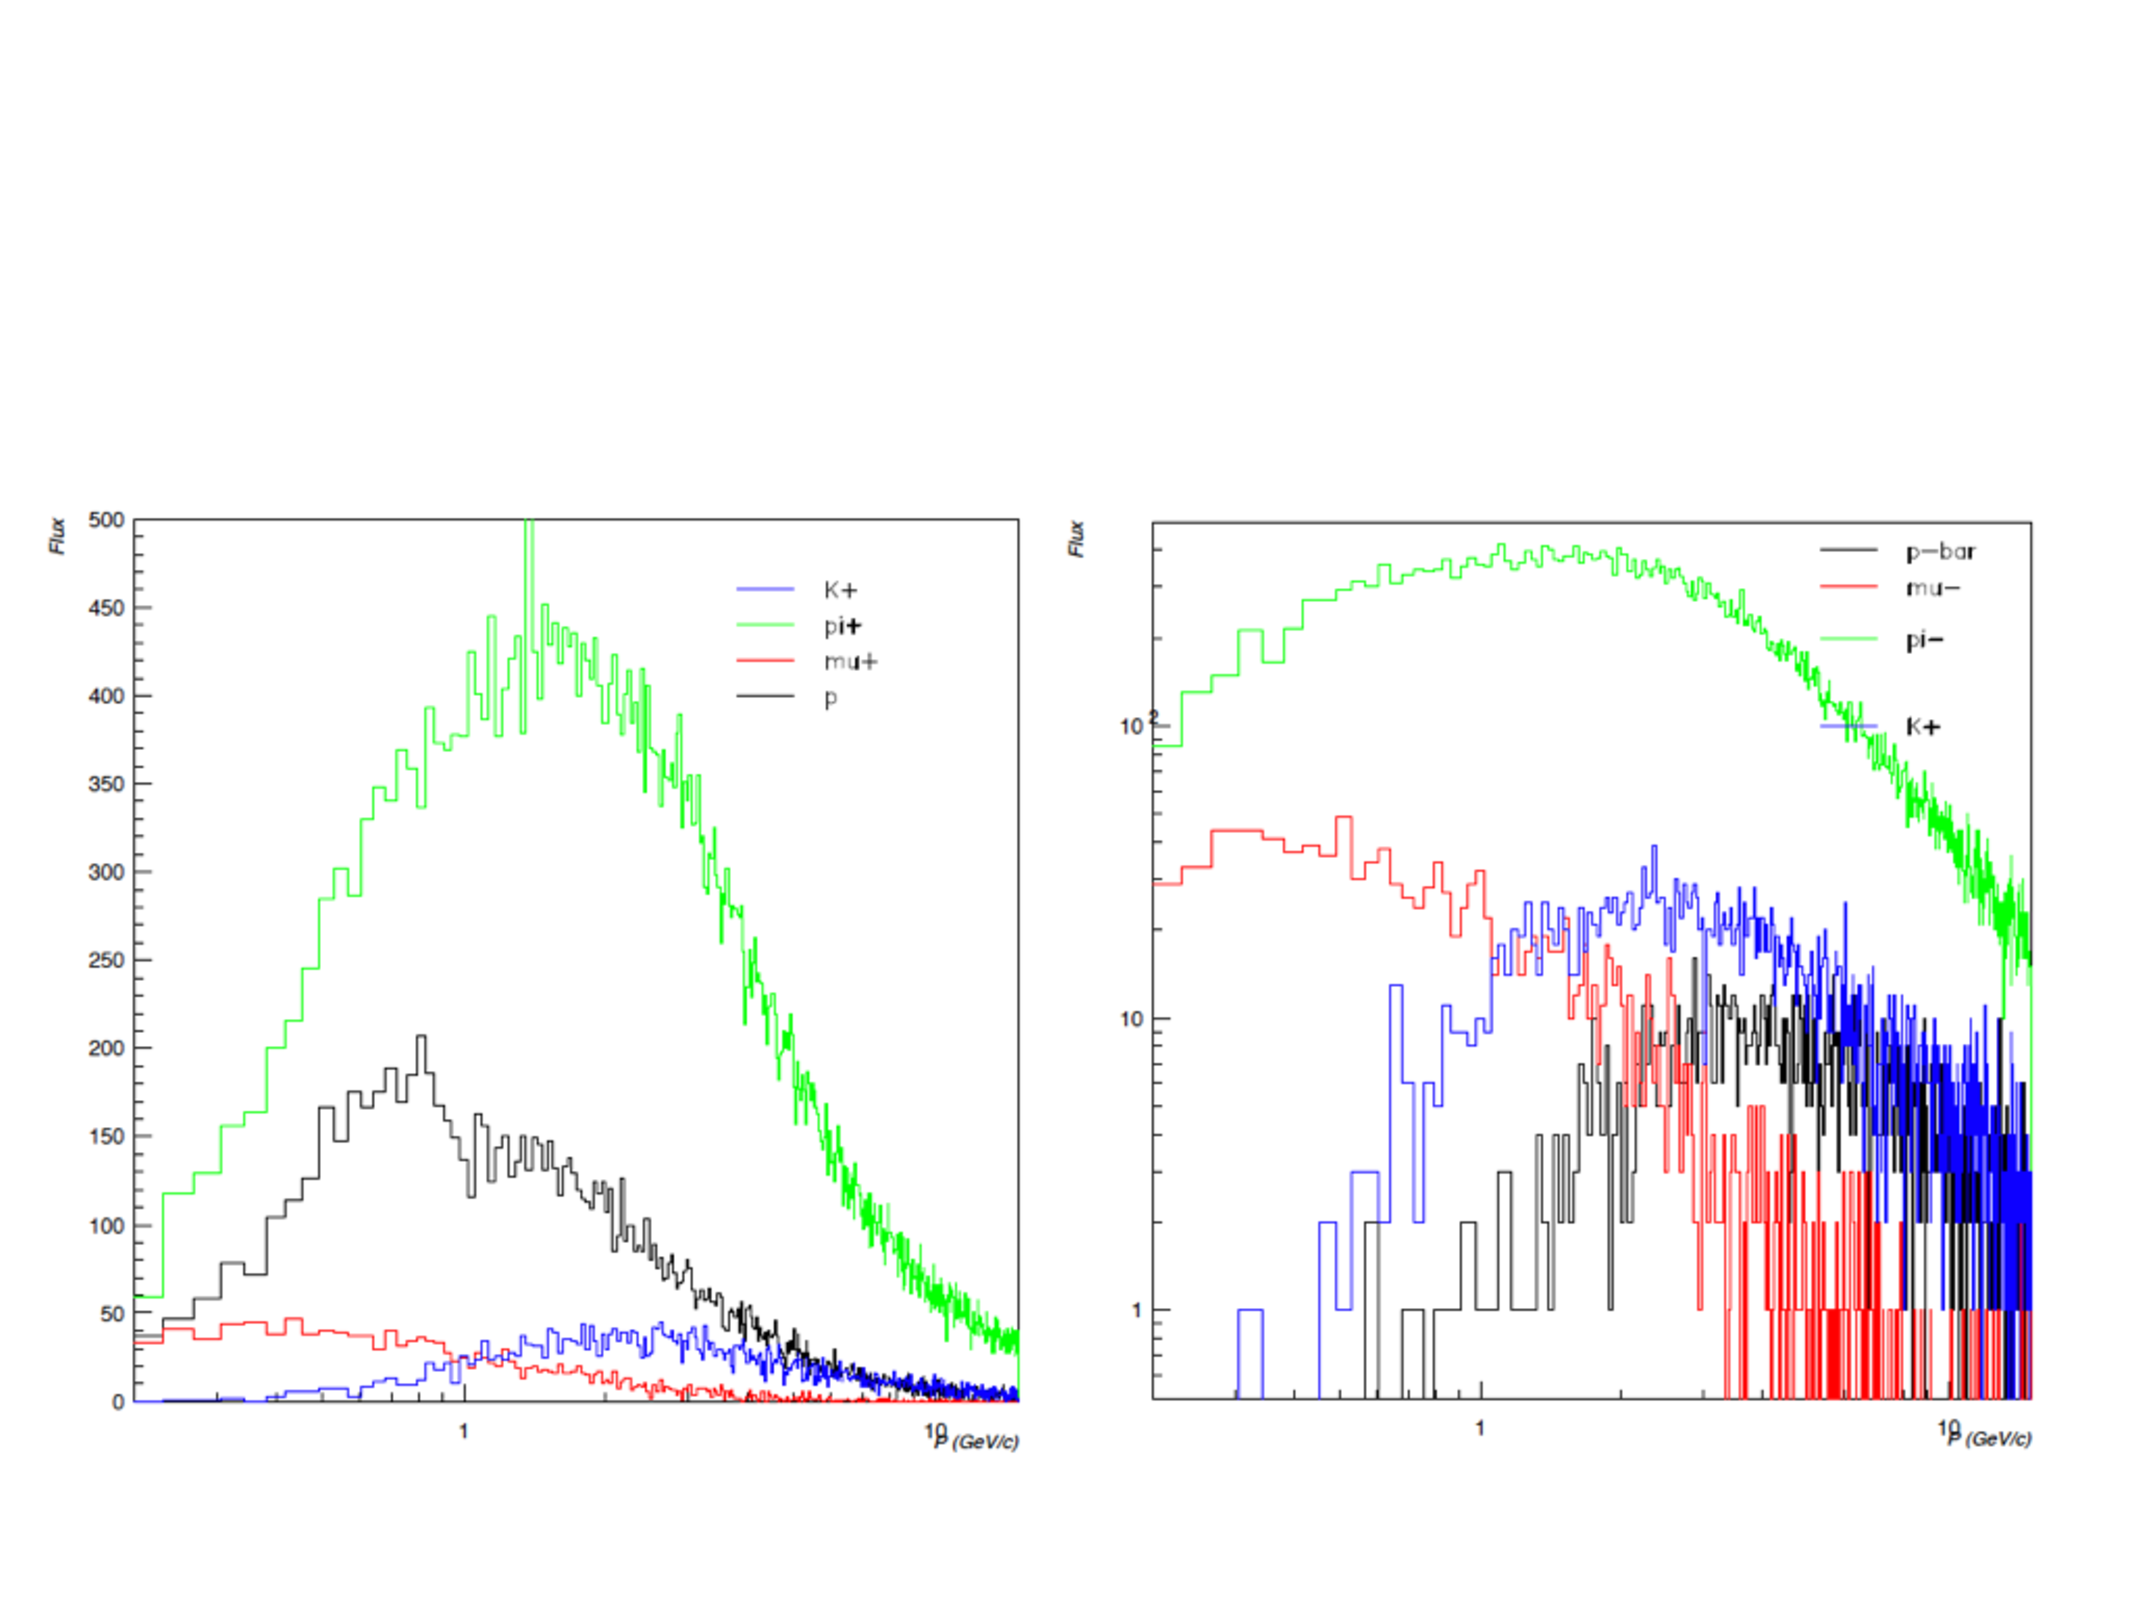
\includegraphics[scale=0.45]{figures/80GeVPion-15cmCuTarget.pdf}
  \caption{Simulation of 100K 80 GeV $\pi^+$ on 15 cm copper target. The figure on the left is for postively charged and the figure on the right is for negatively charged secondary particles from the target. }
\label{fig:PionOnCuTarget}
\end{figure}

To formulate a preliminary beam time request, we assume the hadron beam rates and spectrum as given in Figure~\ref{fig:PionOnCuTarget} with some assumptions about efficiencies and acceptances. For the electron sample, we expect a different optimized beamline setup to produce a pure electron beam with a flux of about 200 Hz. A preliminary run plan is shown in Table~\ref{tab:RunPlan}. The number of spills needed for each momentum bin is driven by the samples highlighted in red or by the requirement that we collect at least 150 spills ($\approx$ 2 hours of beam time) per momentum bin . This proposed plan satifies the requested samples as listed in Table~\ref{tab:runsum}, except for Kaons less than 1 GeV. Most low momentum Kaons produced from the secondary target decay before reaching the liquid argon cryostat. To obtain those samples, we will need to carry out extended runs and trigger exclusively on particles tagged as Kaons by either the time-of-flight or the threshold Cherenkov counters.

\begin{table}[tb]
\centering
\rowcolors{0}{gray!30}{gray!30}
\begin{tabular}{|c|c|c|c|c|c|c|}
\hline
\multicolumn{7}{|c|}{\bf Positive Sample} \\ \hline
\bf $P$ & \bf $\#$ of Spills & \bf Time & \bf $\#$ of $\pi^+$ & \bf$\#$ of $\mu^+$ & \bf$\#$ of $K^+$ & \bf$\#$ of Proton \\ 
\bf (GeV)& & \bf (hours) & & & & \\ \hline
\bf $P$ (GeV) & \bf $\#$ of Spills & \bf Time (hrs) & \bf $\#$ of $\pi^+$ & \bf$\#$ of $\mu^+$ & \bf$\#$ of $K^+$ & \bf$\#$ of p \\ \hline  
\hiderowcolors
0.2&900 &11&\textcolor{red}{\bf 15K} &180K&$\approx$0&160K\\ 
0.3&200 &3 &\textcolor{red}{\bf 15K} &30K &$\approx$0&50K \\
0.4&150 &\textcolor{red}{\bf 2} &22K &18K &$\approx$0&32K \\ 
0.5&150 &\textcolor{red}{\bf 2} &26K &12K &$\approx$0&38K \\
0.7&150 &\textcolor{red}{\bf 2} &40K &10K &$\approx$0&45K \\
1  &350 &4 &120K&\textcolor{red}{\bf 10K} &$\approx$0&65K \\
2  &600 &8 &320K&\textcolor{red}{\bf 10K} &3K        &130K\\
3  &500 &6 &290K &\textcolor{red}{\bf 5K} &7K        &70K \\
5  &1800&23& 1M &\textcolor{red}{\bf 5K}  &5K        &270K\\
7  &1200&15&660K&\textcolor{red}{\bf 6K}  &3K        &120K\\
\hline \hline
\multicolumn{7}{|c|}{\bf Negative Sample} \\ \hline
\showrowcolors 
\bf $P$ & \bf $\#$ of Spills & \bf Time & 
\multicolumn{2}{|>{\columncolor[gray]{0.83}}c|}{\bf $\#$ of $\pi^-$ }& 
\multicolumn{2}{|>{\columncolor[gray]{0.83}}c|}{\bf$\#$ of $\mu^-$ } \\ 
\bf (GeV)& & \bf (hours) & 
\multicolumn{2}{|>{\columncolor[gray]{0.83}}c|}{}& 
\multicolumn{2}{|>{\columncolor[gray]{0.83}}c|}{} \\ \hline  
\hiderowcolors
0.2&600&8&\multicolumn{2}{|c|}{\textcolor{red}{\bf 15K}} &\multicolumn{2}{|c|}{88K}\\
0.3&200&3&\multicolumn{2}{|c|}{\textcolor{red}{\bf 15K}} &\multicolumn{2}{|c|}{30K}\\
0.4&150&\textcolor{red}{\bf 2}&\multicolumn{2}{|c|}{30K} &\multicolumn{2}{|c|}{18K}\\
0.5&150&\textcolor{red}{\bf 2}&\multicolumn{2}{|c|}{40K} &\multicolumn{2}{|c|}{13K}\\
0.7&150&\textcolor{red}{\bf 2}&\multicolumn{2}{|c|}{50K} &\multicolumn{2}{|c|}{12K}\\
1  &150&\textcolor{red}{\bf 2}&\multicolumn{2}{|c|}{70K} &\multicolumn{2}{|c|}{12K}\\
2  &200&3&\multicolumn{2}{|c|}{135K}&\multicolumn{2}{|c|}{\textcolor{red}{\bf 6K}}\\ 
\hline 
\hline
\multicolumn{7}{|c|}{\bf Electron Sample} \\ \hline
\showrowcolors 
\multicolumn{3}{|>{\columncolor[gray]{0.83}}c|}{\bf $P$} &\bf $\#$ of Spills&\multicolumn{2}{|>{\columncolor[gray]{0.83}}c|}{\bf Time}&{\bf $\#$ of electron }\\
\multicolumn{3}{|>{\columncolor[gray]{0.83}}c|}{\bf (GeV)} & &\multicolumn{2}{|>{\columncolor[gray]{0.83}}c|}{\bf (hours)}&\\
\hline
\hiderowcolors
\multicolumn{3}{|c|}{0.2,0.3,0.4,0.5,0.7,1,2,3,5,7}  & 150 per bin & \multicolumn{2}{|c|}{2 hours per bin} &{140K per bin} \\ \hline
\end{tabular}
\caption{A preliminary run plan. The number of spills needed for a given momentum bin is driven by the samples highlighted in red or by the requirement of at least 150 spills per momentum bin.}
\label{tab:RunPlan}
\end{table}

In addition to the above samples with beam at the nominal position, we expect to take some additional data with the beam entering the TPC at different position and angles. Without a detail beamline design, there are still some uncertainties on the actual beam rates. Based on the information that we have, the total estimated beam time needed to carry out the physics program in this proposal is about 4 to 6 weeks.
 
